\subsection{Misura di lambda}
%
Detta $\Delta l$ la differenza tra i due cammini ottici del sistema in considerazione, si ottiene che per i punti di interferenza costruttiva 
    $ \Delta l = n \lambda $, 
mentre per i punti di interferenza distruttiva
    $ \Delta l = (n + 1/2) \lambda $.\\
Notazioni utilizzate:\\
    $x_e$: posizione dell'emettitore su asse x\\
    $x_r$: posizione del ricevitore su asse x\\
%
\subsubsection{Onde stazionarie}
    Riduciamo l'errore sulla misura guardando lancetta con fattore amplificazione 10x fino all'intorno del max. Una volta al max cambiamo su 30x, per poter individuare il massimo più finemente.\\
   % \textbf{Oss}: qui max e min, quindi metà dell'eperimento di fabry perot (massimi consecutivi)\\
    \textbf{Oss}: questo metodo molto più efficiente di Fabry-Perot. La lancetta non oscilla così tanto e il sistema non è così sensibie alle perturbazioni esterne \\
    Emettitore fisso a $ x = 30.0 \pm 0.1 cm $ dallo zero di riferimento.
    Di seguito riportate le posizioni del ricevitore e tipo di picco corrispondente\\
%
    \begin{table}[H]	
\begin{center}
\begin{tabular}{|c|c|}
\hline
    $x_r$	&	Max/min	\\
    cm	&	-	\\
    $\pm 0.1 $	&	-	\\ \hline
    89.3	&	Max	\\
    90.0	&	Min	\\
    90.7	&	Max	\\
    92.2	&	Max	\\
    92.9	&	Min	\\
    93.7	&	Max	\\ \hline    
\end{tabular}
\end{center}
\end{table}
%
    Detta $d$ distanza tra due massimi successivi o due minimi successivi.
    $$ \lambda = 2d = 2.9 \pm 0.2 cm $$
    errore stimato con propagazione.\\
%
\subsubsection{Interferenza da doppia fenditura}
    Distanza tra le fenditure: $7.5 \pm 0.1 cm$\\
    Otteniamo:
        $$ \lambda = d\sin\theta/n = 2.5 \pm 0.1 cm$$
    errore stimato con propagazione.\\
    %
    Misure effettuate:
    \begin{table}[H]
\begin{center}
\begin{tabular}{|c|c|}
\hline
    Angolo	&	Ordine max	\\
    °	&	n	\\
    $\pm 2$	&	-	\\ \hline
    20	&	1	\\
    44	&	2	\\
    57	&	3	\\
    22	&	1	\\
    47	&	2	\\
    58	&	3	\\ \hline
\end{tabular}
\end{center}
\end{table}
%
\subsubsection{Specchio di Lloyd}
    \textbf{Notazioni e formule}\\
    %inserire immagine
    asse x: tra emettitore/ricevitore\\
    asse y: lungo direzione movimento specchio\\
    Cammino1 quello seguito dall'onda diretta\\ Cammino2 quello seguito dall'onda riflessa\\
    Consideriamo come origine (0,0) il centro del goniometro\\
%
    $y_s$: posizione dello specchio su asse y\\
    Cammino2 = 
        $\sqrt{ x^2_e + y^2_s } + \sqrt{ x^2_r + y^2_s }$\\
%
    Troviamo come risultato:\\
    $$\lambda = 2.7 \pm 0.1 cm$$
    errore stimato come standard error.\\
%
    \begin{table}[H]
\begin{center}
\begin{tabular}{|c|c|c|}
%	
    \multicolumn{3}{c}{Misura 1 con: $ x_e = 37.5 \pm 0.1 cm $ , $ x_r = 32.5 \pm 0.1 cm$}\\ \hline
    $y_s$	&	Ordine	&	$\lambda$	\\
    cm	&	n	&	cm	\\
    $\pm$ 0.1	&	-	&	$\pm$0.1	\\\hline
    15.4	&	2° minimo	&	2.6	\\
    18.8	&	3° minimo	&	2.7	\\
    13.3	&	2° massimo	&	2.5	\\
    17.0	&	3° massimo	&	2.6	\\ \hline
%
    \multicolumn{3}{c}{Misura 2 con: $ x_e = 27.5 \pm 0.1 cm $ , $ x_r = 27.5 \pm0.1 cm$} \\ \hline
%
    $y_s$	&	Ordine	&	$\lambda$	\\
    cm	&	n	&	cm	\\
    $\pm$0.1	&	-	&	$\pm$0.1	\\ \hline
    14.5	&	2° minimo	&	2.9	\\
    17.0	&	3° minimo	&	2.8	\\
    12.5	&	2° massimo	&	2.7	\\
    16.0	&	3° massimo	&	2.9	\\ \hline
\end{tabular}
\end{center}
\end{table}
%
\subsubsection{Parte 4: Interferometro di Fabry Perot}
    Fonti di errore: i supporti degli specchi erano molto sensibili alle più piccole oscillazioni, producento alterazioni dei risultati apprezzabili. Siamo stati attenti a non toccare il tavolo.\\
    Detta $d$ la distanza tra due massimi successivi, si ha che:
        $$ \lambda = 2d = 2.7 \pm 0.2 cm$$
    errore stimato con propagazione.\\
%
    Misure effettuate:\\
    \begin{table}[H]
\begin{center}
\begin{tabular}{|c|c|c|}
\hline
    x specchio2	&	$\lambda$	\\
    cm	&	cm	\\
    $\pm 0.1 $	&	$\pm 0.4$	\\ \hline
    55.2	&	-	\\
    54.0	&	2.4	\\
    52.5	&	3.0	\\
    51.1	&	2.8	\\
    49.8	&	2.6	\\
    48.7	&	2.2	\\
    47.1	&	3.2	\\
    45.7	&	2.8	\\ \hline
\end{tabular}
\end{center}
\end{table}
%
\subsubsection{Interferometro di Michelson}
    Le misure sono state fatte prima muovendo lo specchio L1 lugo l'asse x e poi L2 lungo l'asse y.\\
    \begin{table}[H]
\begin{center}
\begin{tabular}{|c|c|}
\hline
    $ x_{L1} $	&	$\lambda$	\\
    cm	&	cm	\\
    $ \pm 0.1 $	&	$ \pm 0.4 $	\\ \hline
    155.2	&	-	\\
    153.8	&	2.8	\\
    152.3	&	3.0	\\
    150.8	&	3.0	\\
    149.5	&	2.6	\\ \hline
    $ y_{L2}$	&	Lambda	\\
    cm	&	cm	\\
    $ \pm 0.1 $	&	$ \pm 0.4 $	\\ \hline
    84.7	&	-	\\
    86.1	&	2.8	\\
    87.6	&	3.0	\\
    89.1	&	3.0	\\
    90.5	&	2.8	\\ \hline
\end{tabular}
\end{center}
\end{table}
    Risultato:
        $$\lambda = 2\Delta x = 2\Delta y = 2.9 \pm 0.2 cm$$
    errore stimato con propagazione.\\
%
\subsubsection{Diffrazione di Bragg}

Il piano reticolare scelto è la diagonale del cubo.
Per ogni misura, è stato fatto ruotare il cubo di 1 grado e il braccio del ricevitore di 2 gradi (entrambi in senso orario), ed è stata letta l'intensità di corrente rilevata. Di seguito il grafico dei dati sperimentali:

    
    \begin{figure}[H]
    \centering
    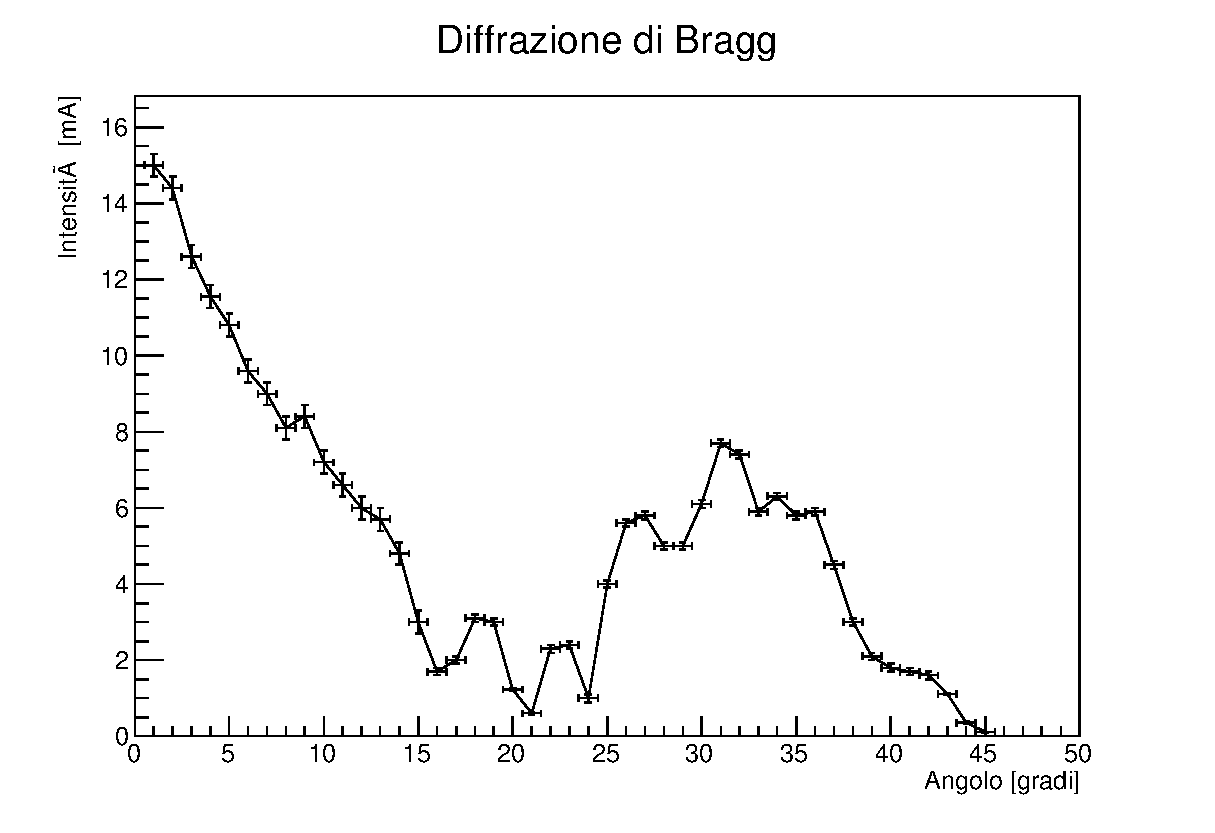
\includegraphics[scale=0.8]{Grafici/O4_P3_Bragg.eps}
    %\caption{}
    \label{fig:O4_P3_Bragg}
    \end{figure} 
%
La distanza tra piani di diffrazione misurata è $d = 2.7$ cm. Il primo massimo ($n = 1$) si trova a $ \theta = 31$ gradi. L'errore sul grado è stato stimato $0.5$ gradi.\\
%
Dalla formula $$2 d \sin(\theta) = n \lambda $$
si ottiene 
$$ \lambda = 2d = 2.8 \pm 0.1 cm $$
In accordo con il valore nominale.
%
